\section{The C Implementation}
\label{sec:cport}

The fixed-point reference model of Section~\ref{sec:fixed} answers
\emph{whether} integer arithmetic preserves the link performance; the C
port (\texttt{cport/}) answers whether the system \emph{fits} a DSP or
microcontroller, and is the code the boards of Section~\ref{sec:radio}
run.  It is portable C99 with no \texttt{malloc} and no floating point
on the signal path (doubles remain on the control plane --- dB values
and timers --- as in the model), and covers the entire feature family:
both FEC families, all three modulations and link modes, the gated
two-stage frequency search, HARQ combining, calibrated LLRs, the
integer SNR estimator, the full link layer with its burst, broadcast
and capability extensions, and a streaming receiver architecture for
MCU deployment.

This section is about the port as a piece of engineering: how
bit-exactness is enforced, how the receiver is restructured to run on a
sample stream, what the extensions beyond the Python reference cost,
how the memory and processor budgets were brought inside an STM32H743,
and what hardening the field campaign forced on the receive front end.
What the boards and their hosts \emph{did} with it --- the two-board
stand, the radio firmware, the USB interface, the SDR path and the
voice mode --- follows in Sections~\ref{sec:radio}
to~\ref{sec:cport_voice}.  Everything measured here is measured on the
channels and stands of Section~\ref{sec:channels}.

\subsection{Bit-Exact Porting Methodology}
\label{sec:cport_method}

Every module is validated against \emph{golden vectors} generated from
the Python fixed-point model (\texttt{gen\_vectors.py}): inputs and
expected outputs are dumped as C headers and compared with
\texttt{memcmp} --- no tolerances anywhere.  Whole transmit frames
(up to 260\,k samples for EXTREME) are compared through 64-bit
FNV-1a hashes over every \texttt{int16} sample, with the first 64
samples embedded verbatim for debuggability.  Two rules keep the
comparison honest:

\begin{itemize}
    \item \textbf{ROMs are dumped, never recomputed.}  Twiddles,
          preamble blocks, pilot symbols, LDPC graph, ladder tables and
          detection kernels all come from the Python model; a C-side
          reimplementation of table generation would risk silently
          diverging in rounding.
    \item \textbf{Width findings are documented, not patched over.}
          Every intermediate that exceeds a naive width estimate
          (Viterbi path metrics, BFP energy sums, the ZC metric's
          Q-scaling) is recorded in \texttt{WIDTHS.md} with its measured
          range, so an RTL implementation inherits the analysis.
\end{itemize}

The suite runs \textbf{177 checks} across eight binaries (primitives
11, bit pipeline 16, TX frames 15, RX demodulation 22, streaming
receiver 11, link layer 80, broadcast 4, USB protocol 18 at the time of
writing), under AddressSanitizer and UndefinedBehaviorSanitizer at the
shipping message geometries as well as the default
(\S\ref{sec:cport_review}).  RX genie vectors are self-hosting: clean frames
are rebuilt by the bit-exact C transmitter inside the test, so only the
Python detection genie (start sample, CFO word) and expected bits are
dumped.

\subsection{Streaming Receiver}
\label{sec:cport_stream}

The frame-at-once reference receiver is impractical on an MCU (it wants
the whole capture in memory), so \texttt{rx\_stream.c} implements a
ring-buffer state machine (\textsc{search} $\rightarrow$ \textsc{zc}
$\rightarrow$ \textsc{header} $\rightarrow$ \textsc{data}) fed in
arbitrary chunks.  The tone-detection stage is necessarily causal and
diverges from the model in two documented ways: block exponents and the
noise floor are windowed (a streaming receiver cannot know the whole
capture's minimum exponent, and the model's whole-capture \emph{median}
floor is acausal), and detection commits on a local metric peak ---
when the above-threshold region ends \emph{and the peak is strong}, or
the argmax stays stable for a full window span --- instead of a global
argmax.  The strength gate ($64\times$ the squared threshold) was
added last: a tone field \emph{entering} the window can produce an
isolated above-threshold spike whose region dies at once, and
committing it anchors two blocks before the real preamble
(\S\ref{sec:voice_onair}, where it cost 0.76\,\% of broadcast
groups on a clean wire).  On the golden corpus
the streaming receiver lands on the identical tone anchor for clean
frames, making everything downstream bit-identical to the
frame-at-once path.

Memory is dominated by sample history, and two measurements shaped the
final architecture:

\begin{itemize}
    \item \textbf{The ring only needs to cover the Zadoff--Chu
          re-anchor lookback, not the preamble.}  The tone stage is
          incremental (each 512-sample block folds into a
          $\approx$540-byte summary; raw tone samples are never
          re-read).  A permanent high-water-mark diagnostic
          (\texttt{rxs\_ring\_hwm}) measured the deepest lookback over
          the corpus at 8\,510 / 32\,318 / 124\,478 samples per mode
          --- the EXTREME figure later fell to 67\,134 when the ZC
          scan was re-anchored (\S\ref{sec:zcscan}).
    \item \textbf{One shared raw ring serves every instance.}  All
          mode-instances listen to the same audio (the preamble root
          self-labels the mode), so concurrent instances write
          identical samples and a single \texttt{int16} ring
          (147\,456 samples, 288\,KB, at this point; 81\,920 samples,
          160\,KB, after \S\ref{sec:zcscan}) replaces per-instance
          analytic rings.  The analytic signal is reconstructed on extraction
          (Hilbert-on-read), bit-identical to the former write-time
          FIR --- and measured \emph{faster}, because the 63-tap filter
          now runs only on consumed regions rather than on every
          sample in every instance.
\end{itemize}

\subsection{Protocol Extensions}
\label{sec:cport_proto}

Three extensions beyond the Python reference address the fixed
per-frame overhead (preamble + header $\approx$0.64\,s in NORMAL mode)
that dominates air time at the top rungs:

\begin{itemize}
    \item \textbf{Selective-repeat burst ARQ.}  Bulk transfers send up
          to a window of frames back-to-back, answered by one bitmap
          acknowledgment (NACK-by-omission).  The two flag combinations
          impossible in the legacy protocol serve as burst frame types,
          so the legacy path is untouched.
    \item \textbf{Extended frames.}  The article's header \texttt{len}
          field counts packet \emph{bits} (255 max
          $\rightarrow$ 27-byte payloads).  An unused header type
          codepoint reinterprets \texttt{len} as payload \emph{bytes},
          allowing 255-byte payloads (2\,076-bit packets) behind a
          single preamble.  Burst fragment size scales with the
          engage-time rung (200\,B at rung $\ge$10, 100\,B at $\ge$7,
          else 25\,B).
    \item \textbf{Streamed burst windows.}  A whole selective-repeat
          window is transmitted behind one preamble and header
          (Sections~\ref{sec:stream} and~\ref{sec:burstwin}) instead
          of one preamble per fragment.  \texttt{tx\_build\_burst}
          waveforms are bit-exact against the fixed-point model, and
          both receivers can follow a burst: the frame-at-once path
          re-runs the recording through \texttt{rxd\_receive\_burst}
          and re-locks on each Zadoff--Chu block, while the streaming
          receiver steps to the next block at its deterministic offset
          via \texttt{rxs\_continue\_burst}.
\end{itemize}

A streamed burst carries only full-size fragments; the short tail of a
transfer always travels as its own frame, because the receiver derives
the message length from that final fragment's own length.  The
acknowledgment request rides on the burst's \emph{first} block as well
as its last, so a peer that cannot follow the stream still answers and
the sender learns by bitmap rather than by waiting out a timeout.

That receive-side continuation is also where the sharpest bug of this
work appeared.  While the streaming receiver is stepping through
blocks it is not running the preamble detector, so a continuation that
does not know where to stop makes the receiver deaf for one block-time
per phantom block.  An early version re-armed its block counter on
every successful block and therefore never learned that a burst had
ended: it chased up to seven blocks that were never sent,
$\approx$12\,s of deafness landing squarely on the peer's next burst,
which timed out and retried indefinitely.  The transmitter marks the
last block of a burst with the acknowledgment request, which is the
stop signal --- qualified as ``set \emph{and} not the first block of
this stream'', since the first carries it too.

Measured on the virtual channel: a 250-byte transfer completes in
3 frames instead of $\approx$20 for stop-and-wait, and a 5\,000-byte
file drops from 211 transmitted frames (legacy) to 45, holding the top
QAM16 rung throughout.  Streaming the window compounds this: a
250-byte transfer at 25-byte fragments takes 4 transmissions streamed
against 13 after falling back to per-frame bursts, and a 14\,kB file
over a $+20$\,dB channel takes 76 transmissions streamed against 187
per-frame.

A fourth extension sits above the protocol rather than inside it.
Nothing in the chain compressed, while every comparable HF system does
--- Winlink's B2F, VARA, and PACTOR all compress before transmitting.
Files are now DEFLATEd whole and the compressed stream is what gets
split into parts; compressing each part separately would discard most
of the ratio, since the dictionary never warms up.  A distinct envelope
magic marks the compressed form, so a peer that predates it sees an
unknown message rather than misparsing a structurally valid one, and
the transmitter falls back to sending raw whenever compression fails to
shrink the payload.  Compression lives at the application layer
precisely so the C port stays dependency-free: an embedded build
substitutes miniz or heatshrink, with plain DEFLATE on the wire either
way.  Measured on a 14\,kB configuration file: 14\,162 bytes to
5\,015 on air, $2.82\times$.  The honest qualification is that
transmissions fell only $1.4\times$ and wall-clock delivery
$1.6\times$, because acknowledgments and the rate-ladder bootstrap do
not compress --- the ratio applies to the part of an exchange that is
payload, not to the exchange.  Supporting endpoints added alongside: a
diagnostic event stream (every TX/RX, timeout, rung change annotated
with the controller inputs that caused it, burst state transitions)
plus a controller-decision snapshot --- which immediately located a
real bug (burst acknowledgment windows systematically timing out and
poisoning the rate controller toward its hard rung-0 fallback; fixed by
forgiving a window's first miss and budgeting the reply air time for
the actual bitmap at a conservative rung) --- and an external
oscillator fine-tune endpoint (VCTCXO DAC / CAT clarifier actuator
driven by the AFC netting loop, with budget clamping, an anchor role,
and a manual override).

\subsection{Memory and Flash Engineering}
\label{sec:cport_memory}

Table~\ref{tab:cport_flash} shows the measured flash footprint
(\texttt{arm-none-eabi-gcc -mcpu=cortex-m7 -O2}, const tables count
into \texttt{.text}).  Three reductions brought the total from an
initial 242\,KB to $\approx$57\,KB with zero runtime cost and
bit-exactness enforced by the golden tests:

\begin{itemize}
    \item \textbf{Preambles stored as their unique periodic blocks}
          (183\,KB $\rightarrow$ 1.3\,KB): each mode's preamble is
          exactly a 32-sample tone block tiled $2T{\times}4$ times, a
          64-sample tone block tiled $T{\times}2$ times, and one
          128-sample ZC tile (whose tail doubles as the cyclic prefix)
          repeated \texttt{sym\_tile} times --- 224 unique samples per
          mode, re-expanded by modulo indexing.
    \item \textbf{Single-table trigonometry} (18.2\,KB $\rightarrow$
          8\,KB): the NCO sine table and all six FFT twiddle arrays are
          exact index-arithmetic views of one 4096-entry cosine table
          ($\sin[i]=\cos[(i+3N/4) \bmod N]$; twiddles at stride
          $N/n$); the generator asserts the identities at dump time.
    \item \textbf{Packed Viterbi traceback} (1 bit per state per step
          instead of a predecessor byte --- the predecessor is
          $(s{\gg}1) + (\mathrm{bit}{\ll}5)$), and \texttt{int32}
          depuncture buffers: extended-frame Viterbi state fell from
          181\,KB to 42\,KB, bit-identically.
\end{itemize}

\begin{table}[H]
    \centering
    \caption{Measured Cortex-M7 flash footprint (all three modes).}
    \label{tab:cport_flash}
    \small
    \begin{tabular}{@{}lrl@{}}
    \toprule
    \textbf{Object} & \textbf{Flash} & \textbf{Dominant tables} \\
    \midrule
    \texttt{fft.o}        & 9.4\,KB  & 8\,KB shared cosine ROM \\
    \texttt{rx\_detect.o} & 10.5\,KB & ZC kernels + detection masks \\
    \texttt{rx\_stream.o} + \texttt{rx\_demod.o} & 16.9\,KB &
                            frequency-search tables \\
    \texttt{ldpc.o}       & 7.2\,KB  & code graph \\
    \texttt{link.o} + \texttt{station.o} & 7.2\,KB & rate-ladder ROM \\
    \texttt{tx.o}         & 3.5\,KB  & 1.3\,KB preamble blocks \\
    \texttt{dsp.o} + \texttt{conv.o} + others & 3.0\,KB & --- \\
    \midrule
    \textbf{Total}        & \textbf{$\approx$57\,KB} & \\
    \bottomrule
    \end{tabular}
\end{table}

\subsubsection{RAM: Making the Cost Follow the Signal, Not the Capture}

The host reference buffers whole captures because a workstation can
afford to: the transmitter assembled a complete frame before clipping
it, the detector materialised its entire search window, and the
demodulator held a whole recording. Linked for Cortex-M7 that came to
roughly 10\,MB of \texttt{.bss}, which is not an optimisation problem so
much as a statement that the reference had never been asked the
question. Five changes took it to 699\,KB, each verified bit-exact
against the golden vectors on both x86 and Cortex-M7.

\textbf{The transmitter generates on demand} (4.3\,MB $\rightarrow$
10\,kB). The waveform is nothing but short periodic blocks repeated:
tone field A is a 32-sample block, tone B is 64, ZC is 128, and a data
symbol is one 128-sample IFFT tile repeated \texttt{sym\_tile} times
behind a CP that is its own tail. So a generator needs one tile, not one
frame. The obstacle is that the clip threshold is a \emph{whole}-waveform
RMS --- the invariant that makes a burst not the concatenation of
separately built frames. Rather than buffer for it, the generator runs
twice: once to accumulate energy, once to emit. It is a pure function of
its inputs, so the second pass reproduces the first exactly.

\textbf{Detection pulls instead of being handed a window} (2.4\,MB
$\rightarrow$ 220\,kB). The ZC scan sweeps up to 70\,688 samples at
EXTREME --- 5.9\,s of audio --- but its \emph{live} span is only
$\mathrm{preamble\_len}+1$: at position $p$ the correlation reads
$[p, p{+}\mathrm{klen})$ and the energy term reads
$m = p-(ng{-}1)\mathrm{klen}$ and $m+\mathrm{preamble\_len}$, which is
the same leading edge because $ng \cdot \mathrm{klen} =
\mathrm{preamble\_len}$ exactly. Likewise the two lag correlations use
lags of 128 and 64 --- not a fraction of the segment --- so they need a
128-sample delay line however long the segment is. A fetch-by-index
source lets the scan read from the raw \texttt{int16} ring that already
holds the audio, derotating on the way out (the phase at index $k$ is
$k \cdot cw \bmod 2^{32}$, which is what makes random access possible).

\textbf{One arena for scratch that is never co-resident} (646\,kB
$\rightarrow$ 129\,kB). Classifying buffers by \emph{lifetime} rather
than by name: the raw ring, the block summaries and the per-symbol LLR
accumulators carry state across calls and cannot be shared, but
everything else is call-scoped, and the phases are strictly sequential
--- detection finishes before the first symbol is demodulated, demod
before decode. One arena sized by the \emph{largest} phase replaces
their sum. The subtlety worth recording is that demod is the largest,
not detection: \texttt{eval\_hyp}'s derotation scratch is live
\emph{while} the symbol samples still are, because it runs inside the
symbol demodulator. Sizing from the buffer list rather than the actual
nesting would have produced silent corruption.

\textbf{Narrowing the sample and soft-decision types.} Measured peaks
across the whole suite justify each: analytic samples 43\,077 (17 bits
$\rightarrow$ \texttt{int32}), LLRs 1\,211\,062 (21 bits), correlation
magnitudes 780\,982 (20 bits). Products of two narrowed values are
widened explicitly --- on Cortex-M7 that is \texttt{SMULL}/\texttt{SMLAL},
the same instruction count as \texttt{MUL}/\texttt{MLA}, so exactness is
free.

\textbf{Per-instance tone summaries} (204\,kB $\rightarrow$ 94\,kB).
Every receiver instance had been given EXTREME's 128-block ring, but an
instance only ever scans its own mode's window: 15/30/120 blocks.

\begin{table}[H]
    \centering
    \caption{Measured Cortex-M7 RAM (\texttt{-Os}, \texttt{--gc-sections},
             linked image referencing only the streaming APIs).}
    \label{tab:cport_ram}
    \small
    \begin{tabular}{@{}lrl@{}}
    \toprule
    \textbf{Component} & \textbf{RAM} & \textbf{Sized by} \\
    \midrule
    Shared raw \texttt{int16} ring & 160\,KB & EXTREME re-anchor
                                               lookback (67\,134) \\
    Scratch arena (RX 3 phases $+$ TX) & 128.5\,KB & EXTREME ZC
                                                     geometry \\
    Tone summaries, 3 instances & 94\,KB & each instance's own mode \\
    LLR buffers (\texttt{int32}) & 24\,KB & 192\,KB with EXT frames \\
    Message store (pooled) & 3\,KB & 12 slots, peak 6 measured \\
    Everything else & 152\,KB & --- \\
    \midrule
    \textbf{Total, three modes} & \textbf{561\,KB} & 793\,KB with EXT
                                                     frames \\
    Transmit-only image & 27\,KB & \\
    \bottomrule
    \end{tabular}
\end{table}

\textbf{Target fit, corrected.} An earlier estimate put the three-mode
station at $\approx$453\,KB and concluded it fitted the STM32H723xG
($\approx$496\,KB usable data RAM) with margin. The linked image does
not: 699\,KB without extended frames, 929\,KB with. The estimate had
costed per-mode summaries while the code gave every instance the
EXTREME count, and assumed a build without EXT frames. Both were
addressed; three further reductions followed, described below and in
Section~\ref{sec:cport_ontarget}, bringing the figure to 561\,KB. The
conclusion is unchanged in kind --- an H743-class device, not the
H723xG --- but the margin is now comfortable rather than absent.  (The
shipping radio firmware then spent part of that margin on 3328-byte
messages and a 16-block stream buffer; its final placement --- station
in SRAM4, ring in D2, LLR buffers in DTCM --- is in
\S\ref{sec:cport_levers}.)

Nor is a single-mode build the way out, though the arithmetic is
tempting. Rung~0 of the ladder is EXTREME, and rung~0 is where both
stations bootstrap, where the controller drops after four consecutive
losses, and where staleness decay lands; rungs 1--3 are ROBUST. A build
without EXTREME cannot acquire a link at all, nor recover one after a
fade --- which is exactly when 64$\times$ tiling earns its cost.
Per-mode sizing is a capability decision, not a memory knob.

Three later reductions are worth separating because each has a
different character. \textbf{The transmitter joined the arena}
(26\,992\,B): a station is half duplex, so the streaming generator's
state --- the one transmit buffer live across calls --- can never
overlap a receive phase in time, and the arena did not have to grow to
hold it. The assumption is checked rather than trusted: receive entry
points stamp an owner tag and \texttt{txs\_pull} refuses to continue a
generator whose state a receive phase overwrote. \textbf{Message
storage was pooled} (161\,280\,B at the demonstrator's settings):
\texttt{station\_t} had given each of the 42 positions that
\emph{could} hold a message its own \texttt{ST\_MSG\_MAX} bytes ---
24 queue slots, 16 delivered-log entries, two current messages --- which
sizes RAM by the number of addressable positions rather than by how many
messages can exist at once. The positions now hold a slot index into one
store of 12; measured peak occupancy is 6, on a 14\,KB file transfer.
\textbf{And the raw ring nearly halved} (128\,KB), for reasons that are
a signal-processing story rather than a bookkeeping one, told in
Section~\ref{sec:cport_ontarget}.

What the exercise changed is less the total than its \emph{shape}.
Nothing in Table~\ref{tab:cport_ram} now scales with frame length,
capture length, or search-window length; every remaining entry is sized
by a property of the waveform. The arena is visibly balanced --- its
receive phases sit within 6\,kB of each other --- which is the signal
that the union has no slack left: it costs the maximum, so no single
phase can be shrunk profitably alone.

\subsection{On-Target Measurement, and What It Corrected}
\label{sec:cport_ontarget}

Every processor figure quoted so far in this report was a
\emph{projection}: analytic multiply--accumulate counts scaled against
an assumed sustained throughput of ``SMLAD-class, $2\times$ overhead
margin: Cortex-M7 at 480\,MHz $\approx$ 400\,MMAC/s''. That assumption
was the weakest line in the document, and it was wrong by a factor of
2.7.

\paragraph{Getting onto the silicon.}
The measurements below were taken on an STM32H743 over JTAG, with an
ESP32 development board as the debug probe: it bit-bangs OpenOCD's
\texttt{remote\_bitbang} protocol, one ASCII character per pin edge,
bridged from a serial port to a socket. This is slow --- 42\,236 edges
per second, so a 52\,KB image takes 84 seconds to download --- but the
probe is the part of the loop that does not need to be fast, and
OpenOCD keeps its own target support. The benchmark runs entirely from
RAM: OpenOCD loads it, points the core at the entry symbol, and reads a
result structure back out of DTCM afterwards. The target's flash is
never written.

Reading the part first settled the memory map, which the datasheet
(DS12110 Table~7) gives only for the H742 and defers otherwise:
\texttt{DBGMCU\_IDC} $=$ \texttt{0x20036450} (revision~V), 2048\,KB of
flash, 512\,KB of AXI-SRAM with \texttt{0x24080000} faulting, and ---
the figure that mattered --- SRAM1/2/3 confirmed \emph{contiguous}
across 288\,KB, which is what permits a single \texttt{g\_raw} to live
there. A trap worth recording: D2 and D3 SRAM are clock-gated and reset
to \emph{off}, so every read of \texttt{0x30000000} fails in a way that
reads as absent memory rather than a disabled clock.

\paragraph{Primitive costs.}
Table~\ref{tab:cport_cycles} gives the measured cycle counts. The
derived MAC throughput is 147\,MMAC/s at 480\,MHz, against the assumed
400 --- so every load projection built on that figure scales up by
$2.7\times$. They still fit: the continuous front end moves from under
1\,\% of a 480\,MHz core to 1.7\,\%, and EXTREME acquisition from a
projected 10\,\% to a measured 27\,\%.

\begin{table}[htbp]
    \centering
    \caption{DWT cycle counts, STM32H743, code in ITCM.}
    \label{tab:cport_cycles}
    \small
    \begin{tabular}{@{}lrr@{}}
    \toprule
    \textbf{Primitive} & \textbf{Cycles} & \textbf{Per unit} \\
    \midrule
    \texttt{fft\_bfp}, 128-point & 91\,376 & 714 / bin \\
    \texttt{hilbert\_analytic} & 3\,970\,631 / 4096 & 969 / sample \\
    \texttt{nco\_derotate} & 159\,763 / 4096 & 39 / sample \\
    \texttt{cordic\_atan2} & 365 & --- \\
    Viterbi, 255 bits rate 1/3 & 2\,465\,972 & 9\,670 / bit \\
    LDPC min-sum, 128 bits, 60 iters & 21\,885\,598 & --- \\
    Complex MAC (correlation inner loop) & --- & 3.27 / MAC \\
    \bottomrule
    \end{tabular}
\end{table}

\paragraph{A memory-attribute trap that looked like an algorithm
problem.}
The same correlation, over byte-identical data, measured 3.27 cycles
per MAC from DTCM and D2 SRAM but 7.52 from AXI-SRAM --- and disabling
the data cache changed the AXI figure not at all. The cause was not the
part: the firmware already resident on the board left an MPU region over
AXI-SRAM with \texttt{TEX=0 C=1 B=0 S=1}, that is, \emph{shareable}.
A Cortex-M7 has no cache-coherency unit, so a shareable Normal region is
effectively uncached. With that MPU disabled all three memories measure
identically. STM32H7 projects mark AXI-SRAM shareable routinely to
sidestep DMA coherency, so this is a live hazard: a misconfigured MPU
costs $2.3\times$ on the acquisition path while presenting as slow code.

The same experiment killed a proposal. Splitting the scratch arena so
that the detection phase lived in DTCM had been designed and costed at
$+126$\,KB before it was measured; the measurement showed it would buy
exactly nothing, because the sliding correlation re-reads 512 samples
per offset and advances by one, so its reuse is $\approx$99.8\,\% and
the 16\,kB data cache absorbs it from any backing SRAM. It was not
implemented.

\subsubsection{The ZC scan, and where its cost actually went}
\label{sec:zcscan}

Acquisition dominates the receiver's processor budget, and within
acquisition the Zadoff--Chu correlation dominates everything else. It is
worth setting out exactly what the scan does, because the eventual
$4\times$ saving came from \emph{where} it looked rather than from how
it computed.

A frame begins with a tone comb of $3T{\cdot}N$ samples ($T$ tone tiles,
$N=128$ bins; 61\,440 samples at EXTREME), followed by one ZC symbol of
$\mathrm{CP}+z_L{\cdot}N$ samples. Detection runs in two stages. The
tone stage folds each incoming 512-sample block into a $\approx$540-byte
summary --- a band energy and, for each candidate frequency shift, the
dot product of the block's spectrum against two masks --- and tracks the
arg-max of that metric. It never re-reads a raw sample. The ZC stage
then correlates the received signal against the known root sequence at
every candidate time offset, taking the peak as the frame boundary.

The critical detail is \emph{when} the tone stage can commit. Partial
overlap crosses the detection threshold roughly a full window before the
true peak, so a decline-from-best rule fires too early; the detector
instead takes the arg-max over the whole above-threshold region and
commits when that region ends. The region ends about one window after
the peak, and the peak is itself one window after the tone field starts.
So at the moment the detector announces a candidate start $c$, the write
head is already \emph{two tone fields} beyond it.

That is a latency, not a cost --- but two consumers turned it into both.
Both anchored at $c$:

\begin{itemize}
    \item the lag-$N$ residual carrier estimate, which correlated the
          tone segment $[c,\,c+2TN)$ --- 40\,960 samples at EXTREME, all
          of them re-read;
    \item the ZC scan, which searched forward from $c$ across the entire
          tone field, 62\,497 candidate offsets, to find a
          symbol that lives at the field's \emph{end}.
\end{itemize}

Both were unnecessary, and each yielded to a different observation.

For the carrier estimate: derotating a signal by a constant per-sample
phase $\theta$ multiplies every lag-$L$ product by the same constant
$e^{-j\theta L}$, because $x'[k]\,\overline{x'[k-L]} =
x[k]\,\overline{x[k-L]}\,e^{-j\theta L}$. The correlation's
\emph{angle} therefore simply shifts by $\theta L$. So the correlation
can be accumulated on \emph{raw} samples, incrementally, one block at a
time as the tone stage already walks past them, and the coarse frequency
word removed at commit as a single angle subtraction. Nothing is
re-read. Checked against the original path on a real EXTREME preamble
across $\pm 120$\,Hz of coarse word, the worst disagreement was 0.0018\,Hz
against a 93.75\,Hz coarse bin.

For the scan: the candidate $c$ is accurate to a fraction of a block.
Measured offsets between $c$ and the true frame start were $+37$,
$-219$ and $-220$ samples for the three modes --- against a search that
swept 62\,497 offsets. The ZC symbol is not somewhere in that span; it
is at a \emph{known} place, the tone field's end, give or take however
wrong $c$ is. So the window is anchored there instead:
%
\begin{align}
    \text{anchor} &= 3TN - m B \\
    \text{window} &= (\mathrm{CP} + z_L N) + 2 m B
\end{align}
%
where $B$ is the detection block length and $m$ is
\texttt{ZC\_ANCHOR\_MARGIN\_BLK}.

\paragraph{What the margin is, and why it is a tuned constant.}
$m$ is the slack allowed on either side of the expected ZC position,
counted in \emph{detection blocks} rather than samples so that it tracks
$B$, which is what the candidate's quantisation error tracks: $c$ is a
block boundary, so it is wrong by at most a block from that alone, plus
whatever the tone arg-max contributes. Measured total error is well
under one block in every mode. The shipped value is $m=8$.

Eight is not a large safety factor in the obvious sense --- it is
roughly $8\times$ the observed error --- but the constant is bounded on
\emph{both} sides, and the bounds are mode-dependent, which is what
makes it delicate. Table~\ref{tab:zcmargin} shows why.

\begin{table}[htbp]
    \centering
    \caption{The anchoring at $m=8$ blocks. The reduction is worth far
             more at EXTREME than at NORMAL, and NORMAL is also the mode
             that constrains $m$ from above.}
    \label{tab:zcmargin}
    \small
    \begin{tabular}{@{}lrrrrr@{}}
    \toprule
    \textbf{Mode} & \textbf{Tone field} & \textbf{$mB$} &
    \textbf{Offsets, was} & \textbf{now} & \textbf{Ratio} \\
    \midrule
    NORMAL  & 3\,840  & 2\,048 & 4\,641  & 4\,129 & 1.1$\times$ \\
    ROBUST  & 15\,360 & 4\,096 & 16\,417 & 8\,225 & 2.0$\times$ \\
    EXTREME & 61\,440 & 4\,096 & 62\,497 & 8\,225 & 7.6$\times$ \\
    \bottomrule
    \end{tabular}
\end{table}

Below the lower bound the window stops covering the ZC reliably and
acquisitions are simply lost: $m=4$ fails the streaming suite. Above the
upper bound something less obvious happens. The margin is subtracted
from the tone field, and NORMAL's tone field is only 3\,840 samples ---
so at $m=16$, $mB = 4\,096$ exceeds it, the anchor clamps to zero, and
the window reverts to searching forward from $c$ while also being wide
enough to reach past the preamble into the data symbols. Data carries
no ZC but does carry structure, and a correlator given more places to
find a peak will eventually find a spurious one. $m=16$ fails the suite
too.

So the valid range is bounded below by the candidate's accuracy and
above by NORMAL's tone field, and the two bounds are only about a factor
of two apart. That is narrow enough that $m$ should be treated as
measured rather than chosen: the sweep below is the instrument, and it
should be re-run if the value is ever moved.

Table~\ref{tab:zcmargin} also explains where the saving actually comes
from. The reduction is worth 7.6$\times$ at EXTREME and essentially
nothing at NORMAL --- which is exactly the right shape, because EXTREME
is the mode whose acquisition dominates the processor budget, and
NORMAL's was never the problem.

\paragraph{What this bought, and what it did not.}
Table~\ref{tab:cport_stages} gives the whole-frame measurement, taken by
piping the streaming transmitter directly into the streaming receiver on
the target so that no buffer ever holds a frame.

\begin{table}[htbp]
    \centering
    \caption{One EXTREME frame (43.5\,s of audio) on an STM32H743,
             before and after the two re-anchorings. Decoded CRC-clean
             in both cases.}
    \label{tab:cport_stages}
    \small
    \begin{tabular}{@{}lrrr@{}}
    \toprule
    \textbf{Phase} & \textbf{Before} & \textbf{After} & \textbf{\% of a
    480\,MHz core} \\
    \midrule
    Tone search & 94.6\,Mcyc & 103.6\,Mcyc & 3.7 \\
    \textbf{Acquisition} & \textbf{4\,050.4} & \textbf{1\,018.0} &
        \textbf{41.8} \\
    Demodulation & 809.0 & 856.8 & 5.5 \\
    \midrule
    \textbf{Whole frame} & \textbf{4\,954.0} & \textbf{1\,978.5} &
        \textbf{9.5} \\
    \bottomrule
    \end{tabular}
\end{table}

Two consequences, and one clarification that matters.

The processor cost of a frame fell from 23.7\,\% of a 480\,MHz core to
9.5\,\%, and acquisition specifically by $4\times$. The tone stage pays
10\,\% more --- 9\,Mcycles, for the per-block correlation it now
maintains --- to save 3\,032. More importantly the burst now runs in
\emph{real time}: before, acquisition needed 8.44\,s of processor inside
a 5.08\,s window and fell behind, catching up afterwards out of the ring;
now it needs 2.12\,s and keeps up with $2.4\times$ headroom.

The ring shrank with it, and for two reasons at once. Its depth is set by
how far back the receiver reaches, which was two tone fields and is now
one plus the search margin: 124\,478 $\rightarrow$ 67\,134 samples at
EXTREME, measured identically on host and target. And because the
processing lag is gone, that reach-back no longer has a backlog added to
it --- previously the two summed to 164\,810 against a 147\,456-sample
ring, an overrun; now 67\,134 sits inside 81\,920 with 14\,786 spare.
288\,KB of RAM became 160\,KB.

\paragraph{The clarification: this is not a decoding improvement.}
It is tempting to read a $4\times$ acquisition saving as better
reception, and it is not. The frames that decoded before still decode,
bit-identically; the frames that failed before still fail. Nothing in
the demodulator, the equaliser, the LLR calibration or the decoders was
touched, and no sensitivity figure in this report moves. What changed is
the \emph{cost} of finding a frame --- processor cycles and the RAM to
buffer the search --- not the probability of finding one. The honest
statement of the benefit is that the same reception now fits on a
smaller, cheaper part with headroom to spare, which is a deployment
result rather than a link-budget one.

There is a plausible argument that narrowing the search should also
\emph{reduce} false locks, since a spurious correlation peak now has
8\,225 places to hide instead of 62\,497 --- but that is a hypothesis,
not a measurement, and it is not claimed here.

\paragraph{Does the narrower search cost sensitivity?}
Cutting a search from 62\,497 candidate offsets to 8\,225 is exactly the
kind of change that trades sensitivity for cost without announcing it,
and the existing C suite could not answer the question --- its only
noisy case is NORMAL at $-5$\,dB against stored samples. The A/B was
therefore built: both arms compile from one source (a switch restores
the original anchor and window) and run over \emph{byte-identical}
EXTREME waveforms --- same seed, same Gaussian noise, same carrier
offset --- so the comparison is paired rather than two independent
samples of a noisy quantity.

Over a wide sweep at 60 trials per point the two arms decoded 291
frames out of 480 each: identical. At the knee, where the curve is
steepest and any loss would show, Table~\ref{tab:zcab} gives 250 trials
per point.

\begin{table}[htbp]
    \centering
    \caption{Paired A/B of the ZC anchoring at the EXTREME sensitivity
             edge, 250 trials per point, identical waveforms.}
    \label{tab:zcab}
    \small
    \begin{tabular}{@{}lrrr@{}}
    \toprule
    \textbf{SNR} & \textbf{Original} & \textbf{Anchored} &
    \textbf{$\Delta$} \\
    \midrule
    $-11.5$\,dB & 223 (89\,\%) & 222 (89\,\%) & $-1$ \\
    $-12.0$\,dB & 195 (78\,\%) & 193 (77\,\%) & $-2$ \\
    $-12.5$\,dB & 138 (55\,\%) & 133 (53\,\%) & $-5$ \\
    $-13.0$\,dB & \phantom{0}58 (23\,\%) & \phantom{0}61 (24\,\%) &
        $+3$ \\
    \midrule
    \textbf{Total} & \textbf{614/1000} & \textbf{609/1000} &
        \textbf{$-5$} \\
    \bottomrule
    \end{tabular}
\end{table}

Half a percentage point, with deltas of mixed sign. The curve falls
$\approx$43 points per dB through that region, which bounds any
sensitivity difference at \textbf{$\approx$0.01\,dB} --- two orders of
magnitude below the $\approx$0.5\,dB effects this report treats as real,
such as the gated coarse search or the streaming resync. And
\textbf{noise-only false alarms were zero in 250 runs for both arms},
against the 0/20 the original detection thresholds were tuned to
(Section~\ref{sec:sync}).

The SNR reference here is the full-band RMS of the transmitted
waveform, which reads roughly 9\,dB pessimistic against the convention
used elsewhere in this report; it is irrelevant to a paired comparison,
where what is measured is two arms on the same input rather than an
absolute sensitivity.

One qualification survives. The margin is a \emph{tuned} constant:
eight blocks passes every streaming test, four fails, and sixteen fails
as well --- at sixteen the anchor clamps to zero for NORMAL and the
window re-admits data symbols, which is a false-lock risk. The value is
not arbitrary and should not be moved without re-running the sweep.

\subsection{Hardening: the Stress Campaign and a DC-Blind Front End}
\label{sec:cport_harden}

With streamed bursts working, an 8\,kB incompressible transfer --- 35
console parts, the largest the boards had attempted --- was put through
the link as a stress test, and sustained load surfaced what a
six-part file never could. Three more failures fell out, each again
convicted by measurement, and the campaign ended in a change of
philosophy rather than another patch: the receiver's front end is now
DC-blind by construction, and its reliability is enforced by a test
gate instead of by luck.

\paragraph{Frames longer than every carrier-sense time constant.}
Fragment size is fixed when a burst transfer engages, so a transfer
engaged at rung~10 with 203-byte fragments that collapsed to rung~0
sent \emph{224-second} EXTREME frames. Carrier sense cannot survive
that: the noise floor's climb crosses the busy threshold after about
176\,s of continuous signal, and the rebase re-baselines at 300\,s ---
either way the peer eventually declares the channel idle and keys over
the frame, which times it out, keeps the rung at zero, and makes the
next frame another 224 seconds. A death spiral with both boards
perfectly healthy. The fix is structural: \texttt{poll\_tx} now
\emph{disengages} a burst whose next fragment would exceed 45\,s of air
at the rung the link actually has (diagnostic \texttt{BURST\_REFRAG});
the message falls to the legacy path, whose payloads are air-time
capped, and the burst re-engages with honestly sized fragments when the
ladder recovers. Streams get the same refusal, and the rebase window
rose to 300\,s --- above the worst frame the station can now emit, not
above demoapp's.

\paragraph{The boot latch.} Gating only the carrier-sense \emph{feed}
for ADC warm-up left the measured mean at zero, and the busy check ---
called every millisecond from boot --- read that zero and snapped the
noise floor to its clamp; a genuinely quiet wire then read ``busy''
forever. The evidence was exact to the millisecond: both boards' first
key-ups ever landed at \texttt{ms=300031} and \texttt{ms=300029} ---
the rebase window precisely, and a collision, two stations going
deaf-mute together at boot. The warm-up gate now covers the consumer
too.

\paragraph{The wire that was never broken.} The campaign's longest
detour was a diagnosis this report must retract as instructively as it
was made. The raw capture ring showed one board's ADC flatlined at a
constant 0.81\,V --- and the obvious call, a failed breadboard contact,
fit every symptom: levels that wandered between reads, a link that
healed mid-run and relapsed, a power cycle that ``fixed'' it. The wire
was innocent. The tick only writes the DAC \emph{while transmitting},
so at the end of every frame the pin held the frame's \emph{last
sample} --- anywhere within $\pm$0.9\,V --- until the next
transmission. Decoding never noticed, because the demodulator is
DC-blind (bin~0 is unused); carrier sense reads mean \emph{square}, and
a DAC parked 0.83\,V off mid-rail put a constant $2.7\times10^8$ on the
peer's carrier sense, at a level that changed with every frame's final
sample. One line parks the DAC at mid-rail at transmit end --- and the
8\,kB transfer promptly completed, byte-exact, in 255\,s.

\paragraph{The lesson, made structural.} A receiver that any input
operating point can break is a lab demo, not a receiver. Two changes
make the property hold by construction rather than by bug-fix
(Figure~\ref{fig:rxfrontend}):

\begin{figure}[htbp]
    \centering
    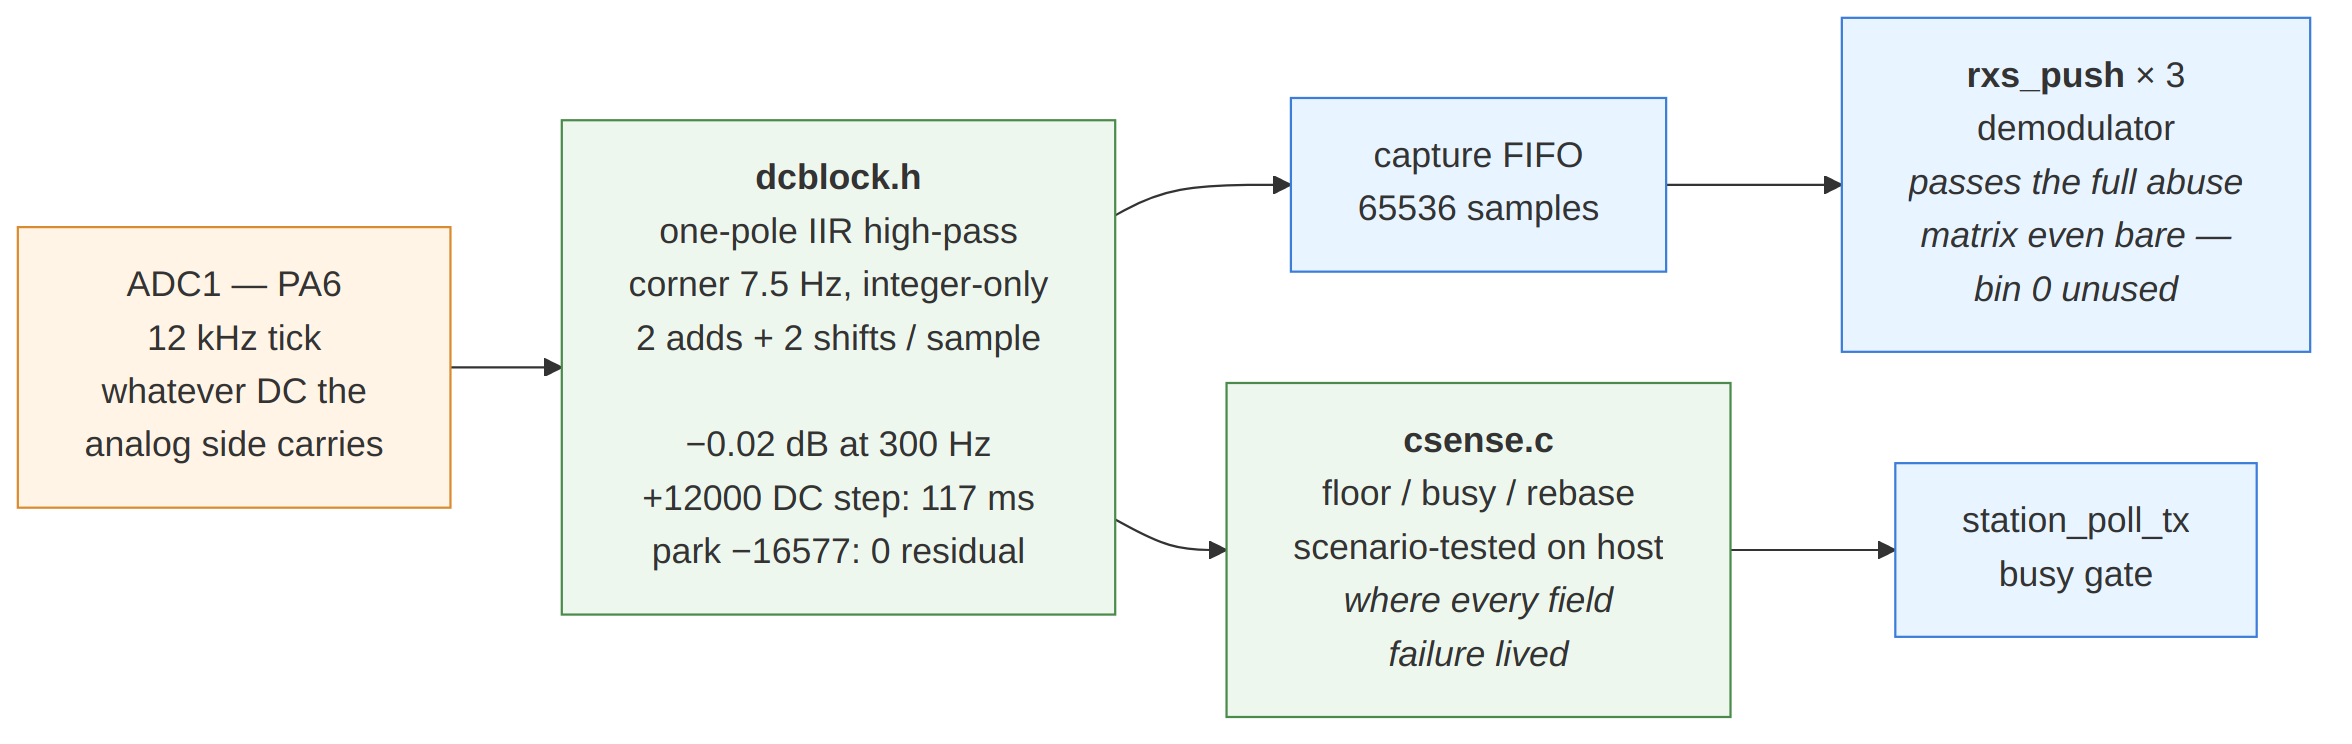
\includegraphics[width=\textwidth]{images/rx_frontend.png}
    \caption{The DC-blind front end. One integer high-pass at the input
             makes every consumer indifferent to the analog operating
             point; carrier sense --- where every field failure of the
             campaign lived --- is a shared module with a host scenario
             suite.}
    \label{fig:rxfrontend}
\end{figure}

First, every ADC sample passes a one-pole IIR high-pass
(\texttt{dcblock.h}: a leaky-integrator DC tracker subtracted from the
input, integer-only, two adds and two shifts per sample) \emph{before}
the capture FIFO and carrier sense. The corner sits at 7.5\,Hz, two
decades under the band: measured, the filter costs $-0.02$\,dB at
300\,Hz, absorbs a $+12\,000$-LSB DC step in 117\,ms, and leaves zero
residual on the measured park level after one second. Whatever DC the
analog side carries --- a parked peer, the bias network that
AC-coupling capacitors would need, a ground offset between boards ---
is now a non-event, which also clears the way for the capacitor
hardware option.

Second, carrier sense moved out of the firmware into a shared module
(\texttt{csense.c}) precisely so it could be \emph{tested}, and
\texttt{make robust} is the resulting reliability gate. Its decode half
drives the burst harness through an input-abuse matrix --- static DC to
$\pm$18\,000 LSB, DC steps, $2.5\times$ clipping, 50\,Hz hum, impulse
clicks, stuck-converter dropouts, all at once, at 5\,ppm of clock
offset --- and its verdict reframes the campaign: \emph{the
demodulator passes the entire matrix even without the blocker.} Every
field failure lived in carrier sense. So carrier sense gets the
scenario half: boot into a quiet wire must read idle within 5\,s (the
latch), the parked DC must read idle through the blocker and
demonstrably latches bare (why the blocker is not optional), a 45-second
frame --- the new maximum --- must hold busy end to end, frame/gap
cycles must track, and a DC step may cost at most a 2-second transient.
Seven scenarios, each a replay of a measured failure; the gate fails on
every bug this campaign found, had it existed a day earlier.

\begin{table}[H]
    \centering
    \caption{The stress campaign, by the numbers. All figures measured
             on the boards or by the host gate.}
    \label{tab:harden}
    \small
    \begin{tabular}{@{}lll@{}}
    \toprule
    \textbf{Quantity} & \textbf{Measured} & \textbf{Note} \\
    \midrule
    8\,kB transfer, final firmware & \textbf{241\,s, byte-exact} & 35
        parts, 36 bitmap acks, 5 timeouts \\
    Same, before the DC blocker & 255\,s & 8 timeouts \\
    Worst pre-fix frame & 224\,s of air & 203-byte frag at rung 0 \\
    Floor climb crosses busy & $\approx$176\,s & why frames are capped
        at 45\,s \\
    Boot-latch key-ups & \texttt{ms} 300031 / 300029 & the rebase
        window, both boards \\
    DC blocker passband & $-0.02$\,dB at 300\,Hz & corner 7.5\,Hz \\
    DC step absorption & 117\,ms & $+12\,000$ LSB \\
    Abuse matrix, demodulator bare & \textbf{8/8 blocks, all rows} &
        DC $\pm$18k, clip, hum, clicks, dropouts \\
    CS scenario suite & 7/7 & each a measured field failure \\
    \bottomrule
    \end{tabular}
\end{table}

\subsection{Calibrating the SNR Estimate}
\label{sec:cport_snrcal}

The chat transcripts from the two-board stand exposed one more defect,
subtler than anything the stress campaign found because nothing
\emph{failed}: messages were delivered, but the rate ladder whipsawed
--- \texttt{rung 10 $\to$ 0 $\to$ 8} with zero losses --- and every
bootstrap climb crawled. The tell was in the diagnostics: EXTREME
frames reported $+0.5$\,dB on a wire that NORMAL frames reported at
$+12$\,dB.

A host sweep of all seven (mode, modulation) combinations the ladder
emits found the mechanism (Figure~\ref{fig:snrcal}, left). The integer
estimator derives SNR from LLR moments, and LLRs \emph{rail} at high
SNR --- at roughly the same raw ratio in every BPSK mode. The estimator
then subtracts the mode's tiling gain (6.02\,/\,12.04\,/\,18.06\,dB),
which is correct near the sensitivity knee where the ratio still moves,
but applied to a railed ratio it simply spreads the ceilings apart:
predicted separations 12.04 and 6.02\,dB, measured 11.9 and 6.1.
Modulation adds its own spread. The consequence is quantitative: the
ladder compares these readings against one \texttt{LADDER\_SENS} table,
and EXTREME's $+0.5$ ceiling sits below
$\texttt{SENS}[10..12]+\texttt{MARGIN\_UP}=+3.2..+7.2$\,dB while
NORMAL's $+12.4$ does not --- so a station that had just decoded an
EXTREME frame could never request the top rungs, however clean the
wire, and one dip to rung~0 dragged both stations down after it.

\begin{figure}[htbp]
    \centering
    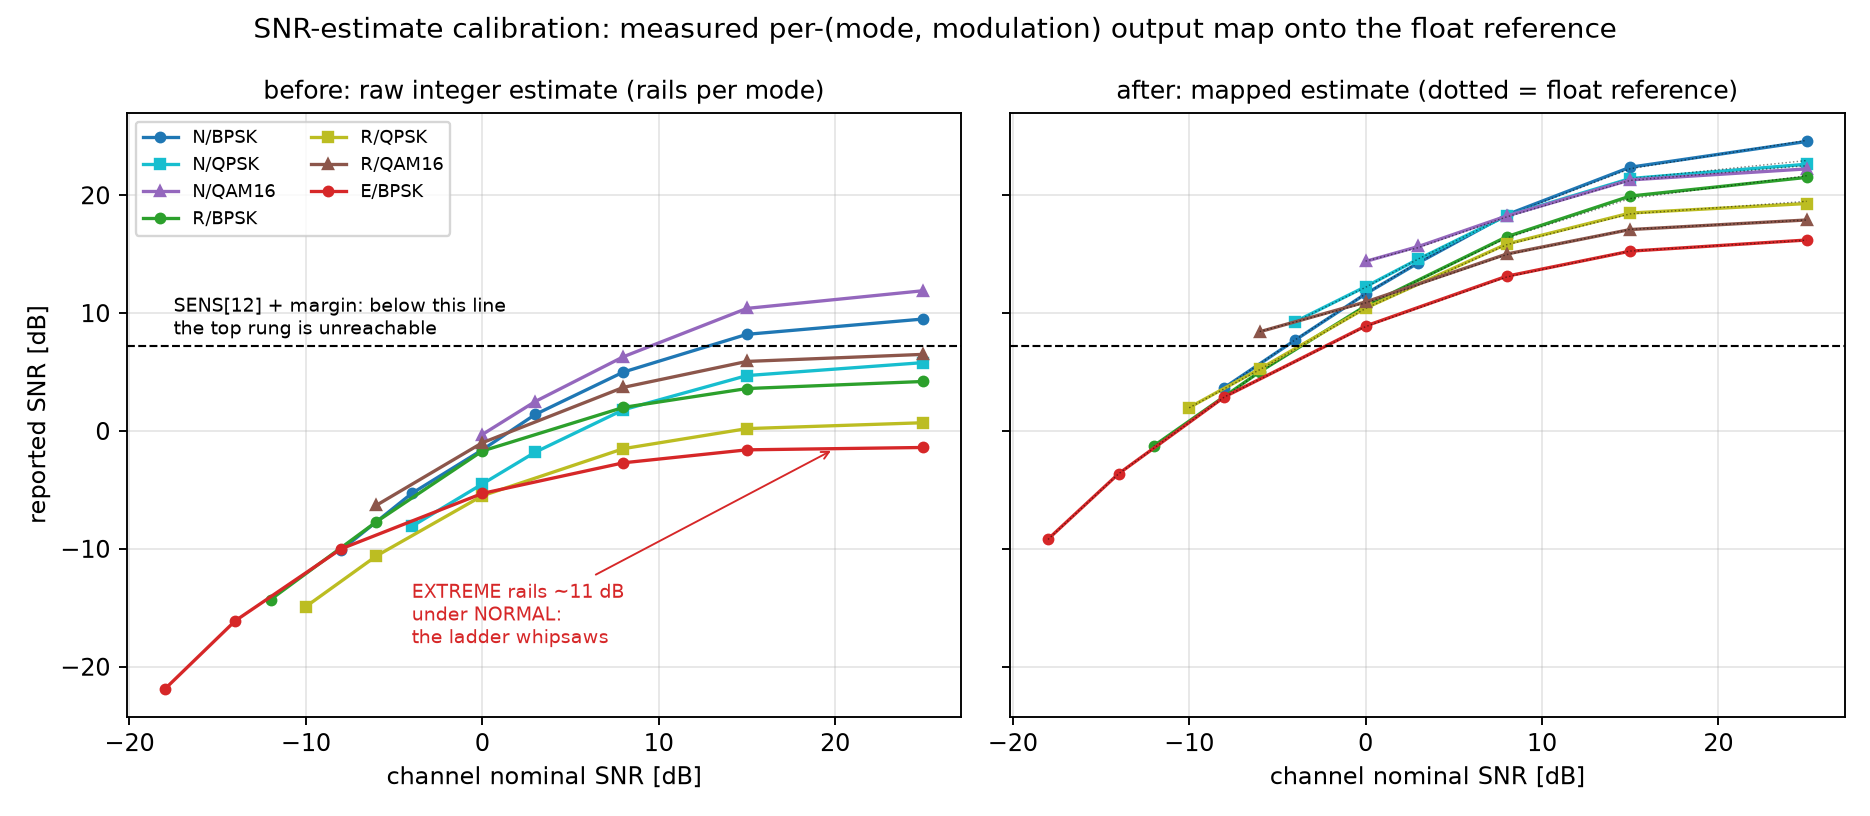
\includegraphics[width=\textwidth]{images/snr_calibration.png}
    \caption{The calibration, before and after. Left: the raw integer
             estimate rails at a per-(mode, modulation) ceiling, and
             EXTREME's ceiling falls below the threshold the top rung
             requires. Right: the mapped estimate, which tracks the
             float reference (dotted) to $\sim$0.3\,dB across the grid.}
    \label{fig:snrcal}
\end{figure}

The fix is a measured map, not a touched constant. Both twins were fed
the \emph{same} noisy waveforms across \texttt{simulate\_channel}'s own
nominal convention --- seven combinations, five to seven nominals each
--- and the resulting (integer estimate, float estimate) pairs became
piecewise-linear output maps. The target is the float estimator
deliberately: it is the reference the rate ladder was system-tested
against, and near the knee the two estimators already agreed (the
fixed-point suite asserted $\pm$2\,dB there), so the map is close to
identity exactly where the existing calibration was right and lifts
only the railed region. The knots live in one place
(\texttt{FixedReceiver.SNR\_MAP}), the generator emits them into
\texttt{rom\_modes.h}, and \texttt{rxd\_snr\_map()} applies them in
both C receive paths --- the parity between twins is by construction,
and the fixed-point suite now asserts the new contract: mapped-integer
tracks float within 3\,dB at nominals $-7/0/{+}15$ (measured medians
0.5\,/\,0.3\,/\,1.2\,dB).

On the boards the change is immediate: EXTREME frames read
$+16.2$\,dB and NORMAL $+20.9..{+}22.5$ on the same wire ---
consistent to $\sim$6\,dB across modes instead of 12 apart, the
residual being the estimators' genuine mode differences --- and the
ladder now climbs $0 \to 11$ in a \emph{single} exchange where it
previously stepped for minutes. The staleness decay's conservative
re-probe after long silence remains, by design.

\subsection{Whose State Is It: a Review, and What It Found}
\label{sec:cport_review}

The operator noticed the boards were busy with nothing attached to
drive them.  They were: one station was keying an acknowledgment-only
frame every second --- 117 frames in 108\,s --- which its peer decoded
and, correctly, never answered.  It had been doing so unattended.

The cause is worth stating precisely, because six more defects turned
out to share its shape.  \texttt{poll\_tx} begins with an early-out:
return unless something is owed, queued, or a capability exchange is
pending.  A flag called \texttt{caps\_kick} bypasses that gate.  But
\texttt{caps\_probe\_wanted()} declines on its \emph{first} line for a
peer whose record is already held --- so the block that would have sent
the probe, and which is the only place that clears the kick, never ran.
Execution fell through to the message path, found no fragment, and
emitted a no-data frame.  Forever.

One bug of that shape justifies looking for others, so the station and
link layers were reviewed along four axes: state that is set and never
cleared, timing and arithmetic, bounds and memory, and ARQ protocol
logic.  Table~\ref{tab:review} is what came back, after each finding was
re-derived against the code and, where possible, measured.

\begin{table}[H]
    \centering
    \caption{Seven defects, and the observation that identifies each.
             None of them announced itself: the counters were healthy,
             or said the opposite.}
    \label{tab:review}
    \small
    \begin{tabular}{@{}p{4.5cm}p{4.3cm}p{4.6cm}@{}}
    \toprule
    \textbf{Defect} & \textbf{Symptom} & \textbf{What it really was} \\
    \midrule
    Burst state outliving its message &
    bytes from before the message pool, encoded and transmitted &
    \texttt{msg\_data()} returned \texttt{pool[-1]} for a released slot \\
    Rung request decaying per \emph{call} &
    ladder collapses to EXTREME after a fade &
    a getter that mutates, called twice per frame \\
    Acks on CAPS / burst frames discarded &
    a retransmission per frame the peer sends, uncounted &
    three branches return before the ARQ retire \\
    Broadcast hold not cleared &
    the second \texttt{bcast} announces and never keys &
    a flag whose only consumer a legitimate path skips \\
    Burst falling through to stop-and-wait &
    duplicate transmission; station busy forever &
    two paths owning one message \\
    Full store acknowledging a drop &
    sender believes a lost message arrived &
    \texttt{done} set before the delivery attempt \\
    Window air time understated 23\,\% &
    a 37\,s transmission under a 30\,s cap &
    a model standing in for the builder \\
    \bottomrule
    \end{tabular}
\end{table}

Three observations generalise beyond this codebase.

\emph{The recurring shape is ownership.}  Almost every entry is state
with a single consumer that some other legitimate path walks around, or
state owned by two things at once.  The repairs are correspondingly
structural rather than local: the burst state is now dropped as a unit
by one function instead of by clearing a flag; an engaged burst owns its
message and the stop-and-wait path will not touch it; the
silence decay is charged against a marker so that asking twice cannot
decay twice; and the window's air time is asked of
\texttt{tx\_burst\_len} rather than modelled from a subtraction that was
never quite right.

\emph{The failures were silent by construction.}  A no-data frame is
never replied to, so the stuck transmitter provoked nothing.  A dropped
message was acknowledged, so the sender saw success.  The doubled decay
moved a number that no counter reports.  This is why the entry point was
an operator noticing a blinking LED rather than any instrument in the
system --- and why the repairs that matter most are the ones that make a
discarded frame say so.

\emph{A sanitizer only sees the path a test walks.}  The
out-of-bounds read has existed for as long as the burst path, and every
suite runs under AddressSanitizer and UndefinedBehaviorSanitizer ---
which do catch it: with the guard removed again as a check, UBSan
reports the index at every message size tried, the default 256 and the
shipping 3328 alike.  What hid it was that no test had ever released a
message while a burst was still engaged, so nothing reached
\texttt{msg\_data()} with a freed slot.  The instrument was sharp
enough; the scenario was missing, and naming it took a review rather
than a tool.

The geometry matters too, but less than it first appears, and in a
narrower way: at the default size that underflow lands \emph{inside} the
neighbouring controller struct, so only UBSan objects and ASan sees
nothing; at the shipping sizes the same expression reads about 3\,kB
outside the object and both fire.  The suites therefore now run at the
shipping geometries as well as the default (\texttt{make
sanitize-ship}), because a gate should exercise the configuration that
ships --- but the lesson that generalises is the first one.
